\documentclass{llncs}
\usepackage{fullpage}

%load needed packages
\usepackage{graphicx}
\usepackage{array}
\usepackage{booktabs}
\usepackage[utf8]{inputenc}
\usepackage{amsmath} 
\usepackage{hyperref}


\begin{document}

\title{Task C: Personal Project}
\subtitle{Replicate og Predicting cervical cancer risk probabilities using advanced H20 AutoML and local interpretable model-agnostic explanation techniques}

\author{Diego De Pablo}
\institute{\email{depablodiego@uma.es} \\
Health Engineering. Málaga University.}

\maketitle 

\vspace{1cm} % Space down the title

\textit{
	Cervical cancer continues to be a significant global health issue. This study aims to replicate, evaluate, and compare the accuracy and efficiency of cervical cancer prediction using machine learning (ML) techniques. We focus on evaluating the approach developed by Sashikanta Prusty\cite{prusty2024predicting}, which combines H2O AutoML with model-agnostic local interpretable model-agnostic explanations (LIME). This hybrid method aims to create highly accurate prediction models while providing interpretable results. Our experimental findings highlight the effectiveness of this approach in accurately predicting cervical cancer cases. By combining H2O AutoML with LIME, we present a robust tool that not only provides accurate predictions but also enhances the understanding of the underlying factors influencing these predictions. This research contributes to the advancement of ML-based solutions for cervical cancer diagnosis and prevention.
	 }



\section{Introduction}

Cervical cancer is the fourth most common cancer among women worldwide and the second most prevalent in developing countries. According to the World Health Organization (WHO), there were 570,000 new cases globally in 2018, with over 90\% of the 311,000 deaths occurring in low- and middle-income countries. India, in particular, has a high cervical cancer incidence rate, ranging from 4.91 to 23.07 per 100,000 women, depending on the region. The primary cause of cervical cancer is persistent infection with high-risk types of Human Papillomavirus, especially types 16 and 18, which are responsible for 70\% of cervical malignancies and precancerous lesions. Other risk factors include early marriage, multiple sexual partners, poor genital hygiene, and the use of oral contraceptives. Although vaccination against Human Papillomavirus and early screening can reduce the burden, challenges remain in low- and middle-income countries due to limited access to screening and qualified healthcare professionals. 

In high-income countries, cervical cancer screening programs, including the Pap test, have significantly reduced mortality. However, in many low-resource settings, the lack of effective screening and healthcare infrastructure continues to contribute to high mortality rates. The application of machine learning has shown promise in improving the accuracy and efficiency of cervical cancer detection, offering a potential solution for resource-constrained environments. Machine learning models can automate the analysis of medical data, thus enhancing early diagnosis and treatment, reducing mortality rates, and making these tools more accessible. 

This study aims to replicate and evaluate a methodology developed by Sashikanta Prusty, which combines automated machine learning with interpretable models to create highly predictive solutions. Specifically, the study uses H2O AutoML, a machine learning platform designed to automate the process of model training and selection, making it easier to deploy highly effective predictive models without requiring advanced expertise. H2O AutoML can automatically train and optimize a variety of models, ranging from decision trees to deep learning models, and select the best performing one for a given task. In addition, this study utilizes the LIME technique, which stands for Local Interpretable Model-Agnostic Explanations. LIME helps to explain the predictions of black-box machine learning models by generating locally interpretable models that approximate the decision boundary of the complex model in the vicinity of a given prediction. This is particularly useful in fields like healthcare, where understanding the reasoning behind a model's decision is crucial for trust and validation. By combining H2O AutoML with LIME, this work aims to improve both the accuracy and interpretability of cervical cancer prediction models, contributing to more effective diagnostic tools in both high and low-resource settings.

\section{Objectives}

\subsection{General Objective}
The general objective of this work is to apply AutoML techniques, specifically the H2O AutoML framework, to automate the machine learning process for predicting cervical cancer. This approach aims to enhance efficiency and accuracy by automating tasks such as data preprocessing, model selection, feature engineering, and model evaluation, ultimately improving the prediction of healthcare outcomes.

\subsection{Specific Objectives}
\begin{enumerate}
	\item To explore the key components of the machine learning pipeline, including data preprocessing, feature engineering, model selection, and evaluation.
	\item To implement the H2O AutoML framework for automating the machine learning process, from raw data processing to the deployment of predictive models.
	\item To evaluate the effectiveness of AutoML in identifying the most appropriate machine learning algorithms and models for cervical cancer prediction.
	\item To examine how neural architecture search and transfer learning are utilized within the AutoML framework to enhance the model's performance on new healthcare datasets.
	\item To compare the performance of models generated by AutoML with traditional machine learning models, focusing on efficiency and accuracy in healthcare applications.
	\item To apply H2O AutoML for predicting cervical cancer outcomes, automating the selection and parameterization of the machine learning models, and assessing the practical benefits for healthcare research and development.
	\item To assess the potential of H2O AutoML in dealing with large, complex healthcare datasets and extracting meaningful insights for better decision-making in the medical field.
\end{enumerate}



\section{Dataset Description}


In this study, two separate cervical cancer datasets were collected from the Kaggle repository, which is publicly available on the Internet. The first dataset consists of 858 samples and 36 features. The 858 samples represent individual patient data, while the 36 features capture various health and demographic factors such as hormonal contraceptives, smoking habits (years), and diagnostic results (e.g., cancer diagnosis, CIN, etc.). These features are primarily responsible for developing abnormal tissue in the cervix, such as the increased risk of Human Papillomavirus (HPV) infection due to behaviors like unprotected sexual intercourse, smoking, and other risk factors. 

The second dataset contains 72 samples and 20 features. These features include factors such as sexual risk behavior, eating habits, personal hygiene, and perceptions of vulnerability. The dataset was preprocessed by removing two features with more than 80\% missing values ("time since first diagnosis" and "time since last diagnosis") and three diagnostic features ("Hinselmann", "Schiller", and "Citology") that provide only indicative results but cannot confirm a diagnosis as definitively as "Biopsy", which was selected as the primary diagnostic tool for predicting cervical cancer. 

After preprocessing, the dimensions of the dataset were reduced to 858 samples and 30 features, which were used for the subsequent prediction model.

\subsection{Dataset Information}
The first dataset, "Cervical Cancer Risk Factors for Biopsy," is obtained from the UCI repository and acknowledges the source. This dataset focuses on the risk factors associated with cervical cancer leading to biopsy examination.

\subsubsection{General Information}
Every year, about 11,000 new cases of invasive cervical cancer are diagnosed in the U.S., although the incidence rate has been declining over the past decades. Despite being the most preventable form of cancer, cervical cancer still claims approximately 4,000 lives in the U.S. and 300,000 globally each year. Early detection through screening, especially the Pap test, has contributed to a 74\% reduction in mortality from 1955 to 1992.

The primary risk factors for cervical cancer include:
\begin{itemize}
	\item \textbf{Age:} 50\% of diagnoses occur in women aged 35-54, with 20\% in women over 65. The median age of diagnosis is 48 years.
	\item \textbf{Socioeconomic and Ethnic Factors:} The risk of cervical cancer is higher in African American and Hispanic women, likely due to socioeconomic factors and lower screening rates.
	\item \textbf{High Sexual Activity:} HPV infection is the leading cause of cervical cancer. Multiple sexual partners, early sexual activity, and HPV infections are major risk factors.
	\item \textbf{Family History:} Women with a first-degree relative (mother or sister) who has had cervical cancer are at a higher risk.
	\item \textbf{Oral Contraceptives:} Long-term use of oral contraceptives increases the risk of cervical cancer, particularly among HPV-infected women.
	\item \textbf{Having Many Children:} Women with multiple pregnancies have an increased risk of cervical cancer, particularly in the presence of HPV infection.
	\item \textbf{Smoking:} Smoking increases the likelihood of developing precancerous changes in the cervix, especially in women infected with HPV.
	\item \textbf{Immunosuppression:} Women with weakened immune systems (e.g., HIV/AIDS) are more susceptible to HPV infections and quicker progression to cervical cancer.
	\item \textbf{Diethylstilbestrol (DES):} Exposure to DES, an estrogen-related drug given to pregnant women from 1938 to 1971, increases the risk of cervical cancer in their daughters.
\end{itemize}

\subsubsection{Additional Information}
The dataset was collected at the 'Hospital Universitario de Caracas' in Caracas, Venezuela, and contains demographic, behavioral, and medical records of 858 patients. Some patients opted not to answer certain questions, resulting in missing data.

\subsubsection{Features}
The dataset includes the following features:

\begin{itemize}
	\item \textbf{Age} (int)
	\item \textbf{Number of sexual partners} (int)
	\item \textbf{First sexual intercourse age} (int)
	\item \textbf{Number of pregnancies} (int)
	\item \textbf{Smokes} (bool)
	\item \textbf{Smokes (years)} (int)
	\item \textbf{Smokes (packs/year)} (int)
	\item \textbf{Hormonal Contraceptives} (bool)
	\item \textbf{Hormonal Contraceptives (years)} (int)
	\item \textbf{IUD} (bool)
	\item \textbf{IUD (years)} (int)
	\item \textbf{STDs} (bool)
	\item \textbf{STDs (number)} (int)
	\item \textbf{STDs: condylomatosis} (bool)
	\item \textbf{STDs: cervical condylomatosis} (bool)
	\item \textbf{STDs: vaginal condylomatosis} (bool)
	\item \textbf{STDs: vulvo-perineal condylomatosis} (bool)
	\item \textbf{STDs: syphilis} (bool)
	\item \textbf{STDs: pelvic inflammatory disease} (bool)
	\item \textbf{STDs: genital herpes} (bool)
	\item \textbf{STDs: molluscum contagiosum} (bool)
	\item \textbf{STDs: AIDS} (bool)
	\item \textbf{STDs: HIV} (bool)
	\item \textbf{STDs: Hepatitis B} (bool)
	\item \textbf{STDs: HPV} (bool)
	\item \textbf{Number of STDs diagnoses} (int)
	\item \textbf{Time since first STD diagnosis} (int)
	\item \textbf{Time since last STD diagnosis} (int)
	\item \textbf{Dx: Cancer} (bool)
	\item \textbf{Dx: CIN} (bool)
	\item \textbf{Dx: HPV} (bool)
	\item \textbf{Dx} (bool)
	\item \textbf{Hinselmann} (target variable) (bool)
	\item \textbf{Schiller} (target variable) (bool)
	\item \textbf{Cytology} (target variable) (bool)
	\item \textbf{Biopsy} (target variable) (bool)
\end{itemize}

%%%%%%%%%%%%%%%%%%%%%%%%%%%%%%%%%%%%%%%%%%%%%%%%%%%%%%%%%55555

\section{Method}


To address the growing demand for machine learning expertise in healthcare, we leverage H2O AutoML to automate the model development process. This enables efficient training of multiple models and selection of the best-performing one. To enhance model interpretability, we employ LIME to elucidate the factors influencing predictions, facilitating trust and understanding in clinical settings. By combining these powerful tools, we aim to develop an accurate and transparent model for cervical cancer prediction.

\subsection{Workflow}

The workflow of this study is designed to leverage H2O’s AutoML capabilities, ensuring an efficient and comprehensive approach to modeling and prediction. Figure \ref{fig:dataset}). shows how it is a different point of view from the traditional one, and directly starts with data preprocessing through H2O AutoML, where data cleaning, imputation, and normalization are performed to ensure a consistent and high-quality dataset. Subsequently, multiple machine learning models are trained using H2O AutoML, which automatically handles model selection, tuning, and evaluation. Model performance is evaluated using key metrics such as AUC, accuracy, and F1 score, and the best performing models are ranked in the AutoML leaderboard.



\begin{figure}[h!]
	\begin{center}  % Usamos el entorno 'center'
		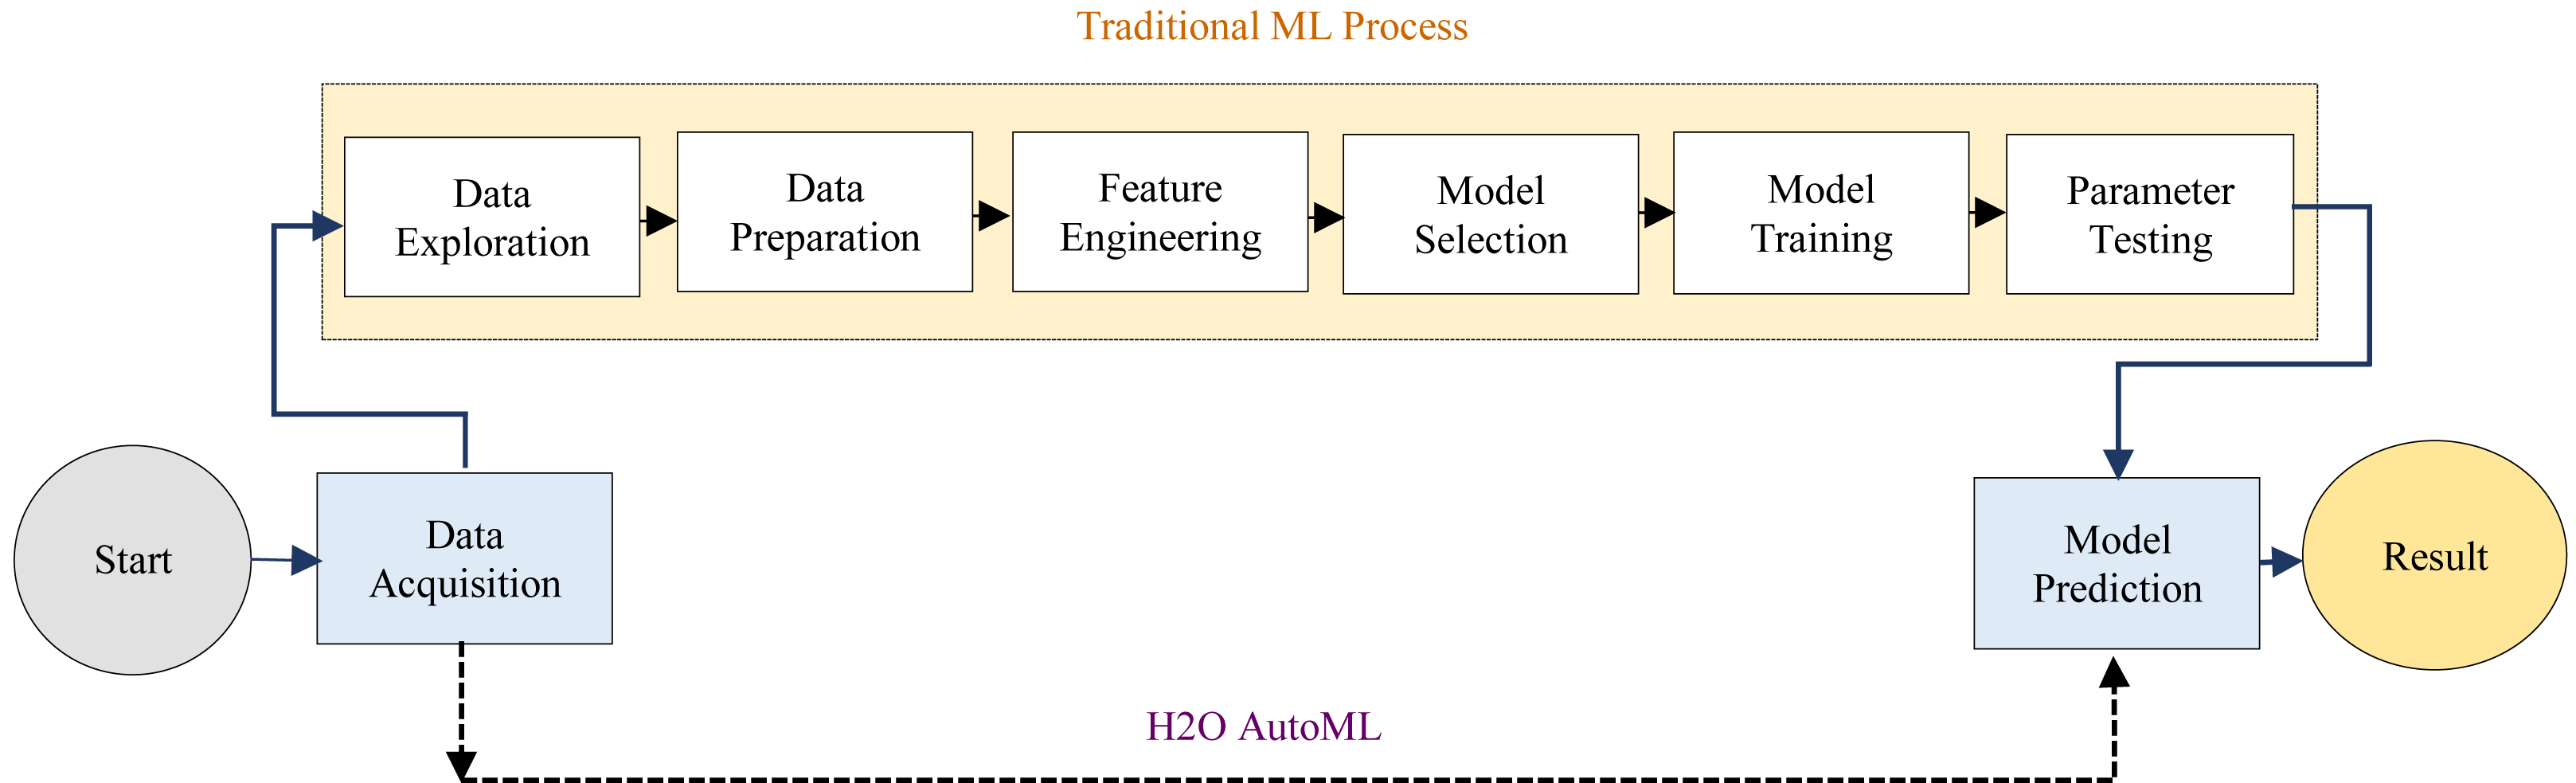
\includegraphics[width=1\textwidth]{images/workflow.png}
		\caption{Differences between the traditional ML and H2O AutoML process.}
		\label{fig:dataset}
	\end{center}
\end{figure}

%\vspace{-20pt} % Ajusta este valor para reducir el espacio

Once the models are trained, the focus shifts to model interpretation. In particular, LIME (Local Interpretable Model-agnostic Explanations) is employed to understand individual predictions, providing insights into the key features driving the model's decision-making. Finally, the best model is selected based on performance metrics, and its predictions are analyzed to derive actionable insights. The entire process is iterative, with regular evaluation of model performance and refinement to achieve optimal results.


\subsection{Handling Missing Values}

In the cervical cancer dataset, missing values are represented by the character \texttt{"?"}. For proper data analysis and processing, it is essential to handle these missing entries appropriately. The first step in this process is to replace all occurrences of the \texttt{"?"} character with \texttt{NaN} (Not a Number), which is the standard representation for missing data in pandas. This conversion ensures that the missing values are correctly recognized and can be handled by subsequent data processing steps.

After replacing the missing values with \texttt{NaN}, we assess the extent of missing data in each feature of the dataset. This is achieved by applying the \texttt{isnull().sum()} function, which counts the number of missing values in each column. This step provides valuable insight into the features that contain missing data and the magnitude of missingness, which is crucial for deciding on appropriate strategies for imputation or removal of data.

To further analyze the distribution of missing data, we visualize its occurrence across the dataset using a heatmap. A heatmap of missing values offers an intuitive and clear representation of the missing data pattern, allowing us to quickly identify whether the missing values are randomly distributed or if there is a specific pattern or correlation between the missing values in different columns. This visualization aids in making informed decisions about how to address the missing data. However, it should be noted that this step is primarily exploratory and does not contribute directly to the model-building process.

\subsection{Data Visualization}

In this section, we delve into the relationships between various risk factors and the biopsy results to gain a comprehensive understanding of the potential variables that could influence the presence of cervical cancer. To uncover these relationships, we employ correlation analysis using three distinct methods: the Pearson correlation coefficient (Fig. \ref{fig:pearson_corr}), the Spearman correlation coefficient (Fig. \ref{fig:spearman_corr}), and Kendall's Tau coefficient (Fig. \ref{fig:kendall_tau_corr}). Each of these methods allows us to examine different aspects of the associations among the numerical variables in the dataset. The Pearson correlation coefficient assesses linear relationships, providing a measure of the strength and direction of linear associations, while the Spearman and Kendall Tau coefficients focus on monotonic and ordinal relationships, respectively. By utilizing these three methods, we can identify both linear and non-linear dependencies between the features, offering a nuanced understanding of how different factors may be interrelated and contribute to the outcome of interest.

In addition to correlation analysis, we enhance our exploratory data analysis (EDA) by generating an automated report using the DataPrep library. This report summarizes key characteristics of the dataset, such as data distributions, measures of central tendency (mean, median), and the relationships between variables, providing a holistic view of the dataset’s structure and identifying any potential data quality issues or trends.

Furthermore, to better visualize the distribution of critical risk factors, we create count plots for variables such as age, number of sexual partners, number of pregnancies, smoking habits, and contraceptive use, all stratified by biopsy results. These visualizations offer a clearer understanding of how these factors might be associated with the presence or absence of cervical cancer, highlighting potential trends or imbalances that could be valuable for further analysis and model development.

\subsubsection{Correlation Matrix}

First, we calculate the correlation matrix to identify any linear relationships between the numerical variables in the dataset. The Pearson correlation coefficient is used to evaluate the strength of linear associations between the features, where values closer to +1 or -1 indicate a strong positive or negative linear relationship, respectively. This matrix helps us to identify potential multicollinearity or redundant variables that may need to be addressed before model training.

\begin{figure}[htbp]
	\centering
	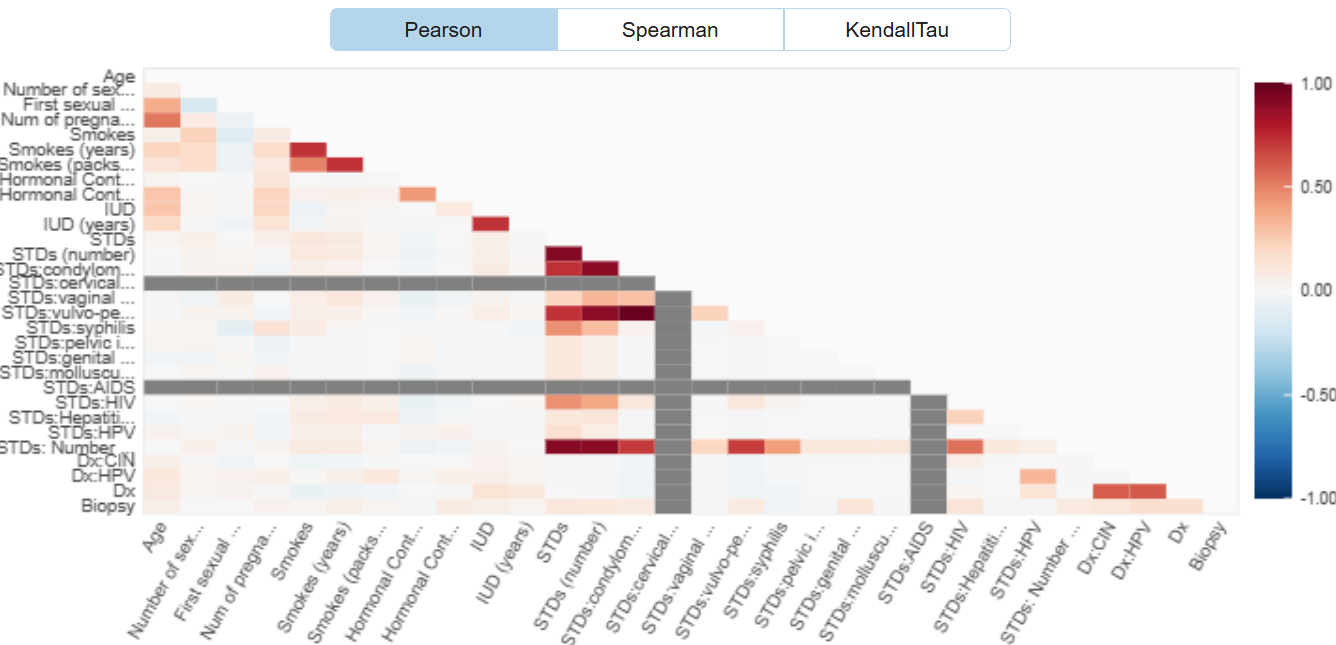
\includegraphics[width=0.7\textwidth]{images/pearson_correlation.png}
	\caption{Pearson Correlation Coefficient Matrix}
	\label{fig:pearson_corr}
\end{figure}


As shown in Fig. \ref{fig:pearson_corr}, the Pearson correlation coefficient matrix highlights the relationships between different numerical variables, allowing us to pinpoint which features are most strongly correlated with each other. These insights are essential for understanding the underlying patterns in the data and for making informed decisions about feature selection in subsequent analysis steps.


Next, we calculate the Spearman correlation coefficient to assess the monotonic relationships between the numerical variables. Unlike Pearson, which only detects linear relationships, Spearman’s method measures the strength and direction of a monotonic relationship, meaning that it can capture both linear and non-linear trends. Spearman's rank correlation is based on the ranks of the values, rather than the raw data itself, making it more robust to outliers and non-linear associations.

\begin{figure}[htbp]
	\centering
	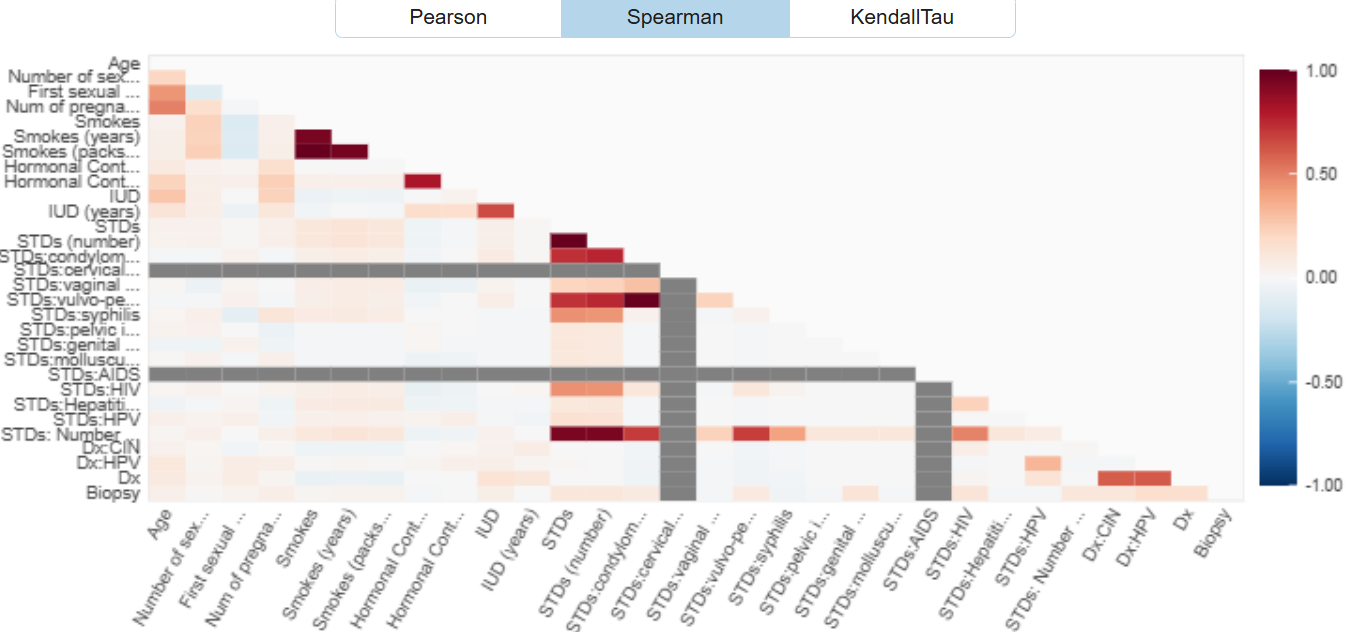
\includegraphics[width=0.7\textwidth]{images/spearman_correlation.png}
	\caption{Spearman Correlation Coefficient Matrix}
	\label{fig:spearman_corr}
\end{figure}

As depicted in Fig. \ref{fig:spearman_corr}, the Spearman correlation matrix reveals how different numerical variables are related in a monotonic manner. Variables with high positive or negative correlations suggest strong monotonic relationships, which can provide insights into underlying patterns in the data, even when those relationships are not strictly linear.

We also calculate Kendall’s Tau to evaluate the ordinal relationships between the variables. Kendall’s Tau is a non-parametric statistic that measures the strength of association between two variables based on the number of concordant and discordant pairs. This method is particularly useful when the data does not follow a normal distribution or when there are ties in the data. Kendall’s Tau tends to be more robust to tied ranks compared to Spearman’s correlation.

\begin{figure}[htbp]
	\centering
	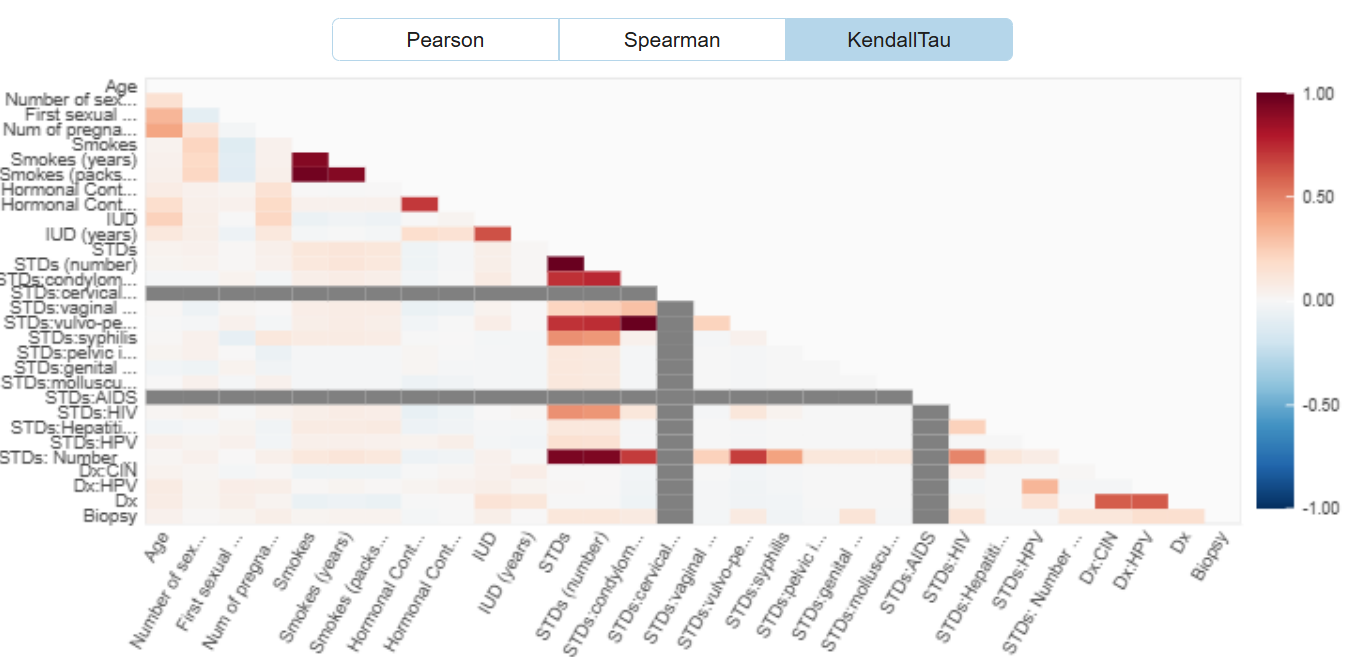
\includegraphics[width=0.7\textwidth]{images/kendall_tau_correlation.png}
	\caption{Kendall Tau Correlation Coefficient Matrix}
	\label{fig:kendall_tau_corr}
\end{figure}

Fig. \ref{fig:kendall_tau_corr} presents the Kendall Tau correlation matrix, which allows us to explore the relationships between variables in an ordinal fashion. Kendall Tau is especially useful when dealing with smaller datasets or when the data contains many tied ranks. Strong correlations indicate that the variables tend to move in the same direction, which may suggest potential predictive factors for the target variable.

While Pearson’s correlation (Fig. \ref{fig:pearson_corr}) measures linear relationships, Spearman (Fig. \ref{fig:spearman_corr}) and Kendall’s Tau (Fig. \ref{fig:kendall_tau_corr}) focus on monotonic and ordinal relationships, respectively. Although Pearson’s correlation is sensitive to linear dependencies, it may not capture complex monotonic trends that Spearman and Kendall Tau can. On the other hand, Spearman’s and Kendall’s Tau coefficients are more appropriate for non-linear, monotonic, or ordinal relationships and tend to be more robust in the presence of outliers or ties in the data.

From the correlation matrices, we observe that Pearson’s and Spearman’s methods often reveal similar relationships, particularly in cases where the data follows a linear pattern. However, Kendall’s Tau tends to produce slightly different results, especially when the data contains many tied ranks or when the relationships between variables are more ordinal in nature.

\subsection{Preparing H2O Dataframes}

\subsubsection{Starting and Connecting to the Local H2O Cluster}

H2O is a powerful set of utilities designed for efficient interaction with the H2O machine learning platform. It provides a robust environment for performing large-scale data analysis, modeling, and machine learning. In this study, we utilized H2O's functionalities to process and analyze our dataset. To begin, we start or connect to a local H2O cluster, enabling us to take full advantage of H2O's parallel processing capabilities.

The connection to the H2O cluster was established using version \texttt{3.34.0.7}, and the cluster was named \texttt{H2O\_from\_python\_Lelin\_scenxd}. The setup was performed using Python version \texttt{3.8.8} running on a Windows 10 operating system. The H2O web UI, accessible through an internet browser, was used for monitoring the cluster and managing operations. Specifically, we utilized Microsoft Edge version \texttt{117.0.2045.60} (64-bit) to connect to the H2O web interface, which provides a convenient and interactive way to track the status of our cluster and perform various tasks such as data importation, exploration, and model training.

\subsubsection{Importing Data into H2O}

Once the H2O cluster was successfully connected, we proceeded to import the dataset into the cluster for processing and analysis. H2O supports a variety of data formats, and the dataset was loaded into an H2O dataframe, a highly efficient structure optimized for distributed computing. This allows us to leverage H2O's machine learning algorithms for large-scale data analysis, without the need to transfer the data to a single machine.

The importation of data into H2O is facilitated by using the \texttt{h2o.import\_file()} function, which is capable of handling large datasets by reading them directly from the local file system or remote storage. The resulting H2O dataframe was then used for subsequent preprocessing, analysis, and model building, ensuring that all operations were performed in a memory-efficient manner across the distributed H2O cluster.

\subsection{Training H2O AutoML}

In this section, we use H2O AutoML to train multiple machine learning models on the cervical cancer dataset and select the best model based on the AUC (Area Under the Curve) metric. This process automates model selection and hyperparameter tuning for efficient training.

\subsubsection{Data Preparation}

We begin by connecting to the H2O cluster and converting the pandas DataFrame into an H2O frame. The dataset is then split into training (75\%) and testing (25\%) sets, and the target column (Biopsy) is converted into a factor for binary classification.

\subsubsection{Model Training}

Next, we initialize the H2O AutoML model, specifying AUC as the optimization metric and limiting the model count to 20, excluding StackedEnsemble models. The AutoML model is trained using the predictors (X) and target (y), with H2O handling model selection, hyperparameter tuning, and evaluation. The best-performing model is selected based on the AUC score.

\subsection{Compare Models and Make Predictions}

\subsubsection{Model Comparison}

After training the models with H2O AutoML, we use the \texttt{explain} function to visually compare their performance on the test set. This comparison highlights the strengths and weaknesses of each model, focusing on the leader model selected by AutoML.

\subsubsection{Model Explanation}

We further explain the behavior of the best-performing (leader) model using the \texttt{explain} function. This helps us gain deeper insights into how the model makes predictions on the test set.

\subsubsection{Making Predictions}

Finally, we use the leader model to generate predictions on the test data. These predictions are then combined with the original test set for further analysis.


The table \ref{tab:model_performance} presents a summary of the performance metrics for the various machine learning models evaluated during the AutoML process. Each row represents a different model, identified by its model number, and the following columns provide key performance indicators:

\begin{itemize}
	\item \textbf{Model Number}: A simplified identifier for each model.
	\item \textbf{AUC (Area Under the Curve)}: Measures the model's ability to distinguish between positive and negative classes, with higher values indicating better performance.
	\item \textbf{LogLoss}: A metric that evaluates the accuracy of the model's probabilistic predictions, where lower values indicate better performance.
	\item \textbf{AUCpr (Area Under the Precision-Recall Curve)}: A measure of model performance with a focus on the positive class, especially useful in imbalanced datasets.
	\item \textbf{Mean Per Class Error}: The average error rate per class, with lower values indicating better classification accuracy.
	\item \textbf{RMSE (Root Mean Square Error)}: A measure of the model's prediction error, with lower values indicating better predictive accuracy.
	\item \textbf{MSE (Mean Square Error)}: The square of the RMSE, which provides an overall indication of the model's prediction error.
\end{itemize}

This table helps compare the relative performance of the models and provides a quick overview of which models performed best across multiple evaluation metrics.


\begin{table}[htbp]
	\centering
	\begin{tabular}{|c|c|c|c|c|c|c|}
		\hline
		\textbf{Model Number} & \textbf{AUC} & \textbf{LogLoss} & \textbf{AUCpr} & \textbf{Mean Per Class Error} & \textbf{RMSE} & \textbf{MSE} \\
		\hline
		1 & 0.66 & 0.25 & 0.12 & 0.41 & 0.25 & 0.06 \\
		2 & 0.66 & 0.25 & 0.11 & 0.36 & 0.26 & 0.07 \\
		3 & 0.66 & 0.59 & 0.14 & 0.37 & 0.26 & 0.07 \\
		4 & 0.65 & 0.32 & 0.14 & 0.39 & 0.29 & 0.08 \\
		5 & 0.64 & 0.30 & 0.14 & 0.41 & 0.26 & 0.07 \\
		6 & 0.63 & 0.43 & 0.10 & 0.38 & 0.36 & 0.13 \\
		7 & 0.63 & 0.28 & 0.17 & 0.40 & 0.25 & 0.06 \\
		8 & 0.63 & 0.34 & 0.12 & 0.39 & 0.31 & 0.10 \\
		9 & 0.63 & 0.52 & 0.10 & 0.38 & 0.30 & 0.09 \\
		10 & 0.62 & 0.37 & 0.11 & 0.43 & 0.33 & 0.11 \\
		11 & 0.61 & 0.25 & 0.09 & 0.40 & 0.25 & 0.06 \\
		12 & 0.61 & 0.54 & 0.10 & 0.42 & 0.30 & 0.09 \\
		13 & 0.60 & 0.55 & 0.10 & 0.43 & 0.29 & 0.08 \\
		14 & 0.60 & 0.45 & 0.09 & 0.39 & 0.38 & 0.14 \\
		15 & 0.60 & 0.32 & 0.13 & 0.39 & 0.26 & 0.07 \\
		16 & 0.59 & 0.27 & 0.09 & 0.42 & 0.26 & 0.07 \\
		17 & 0.56 & 0.25 & 0.10 & 0.43 & 0.25 & 0.06 \\
		18 & 0.54 & 0.34 & 0.14 & 0.43 & 0.28 & 0.08 \\
		19 & 0.53 & 0.32 & 0.10 & 0.45 & 0.26 & 0.07 \\
		20 & 0.41 & 0.26 & 0.06 & 0.49 & 0.26 & 0.07 \\
		\hline
	\end{tabular}
	\caption{Model Performance Summary}
	\label{tab:model_performance}
\end{table}

\subsection{Use LIME to Explain H2O Models}

LIME (Local Interpretable Model-agnostic Explanations) is a technique used to interpret the predictions of complex machine learning models by approximating them locally with simpler, interpretable models. In this study, we apply LIME to the leader H2O model to gain a better understanding of the factors influencing individual predictions.

LIME works by generating a new dataset composed of permuted data points (i.e., data with shuffled feature values) and then obtaining predictions from the black-box model for these new data points. A simple model, such as a linear regression or decision tree, is then trained on this permuted dataset, allowing us to understand the behavior of the original model in the vicinity of the prediction being explained.

In our research, we focus on predicting the probabilities for class labels (either '0' or '1'). We conduct experiments with three different instance values: IDX 100, 120, and 150, each corresponding to different test instances. These experiments generate separate explanation files, which are shown in Figures \ref{fig:IDX100} , \ref{fig:IDX120} , and \ref{fig:IDX150}. For each case, LIME provides insights into which features have the most influence on the model’s prediction.


\begin{figure}[htbp]
	\centering
	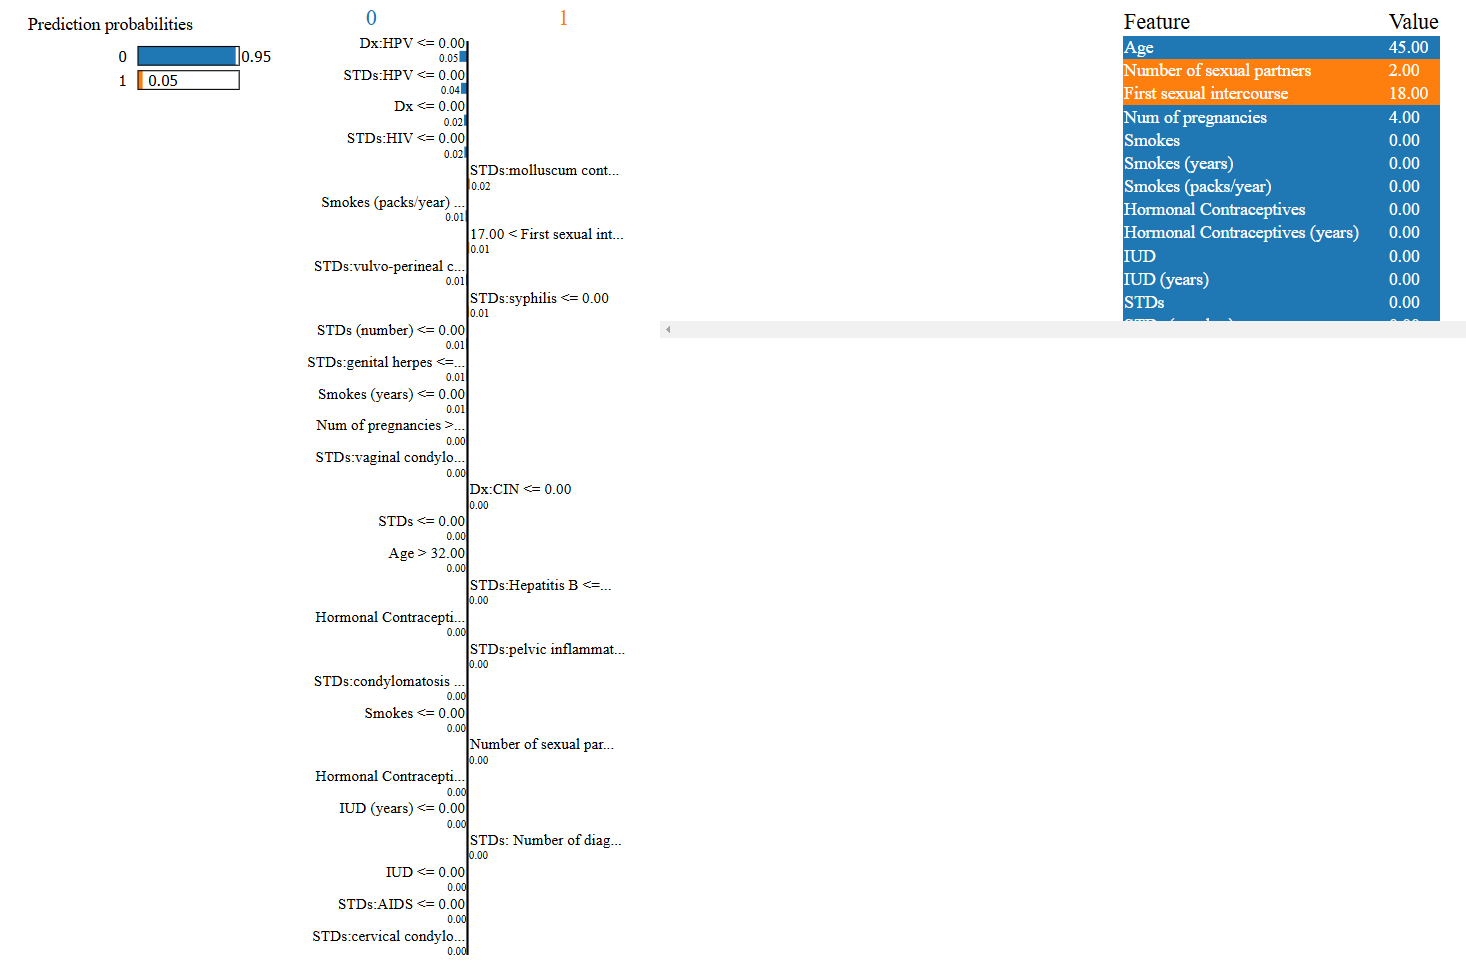
\includegraphics[width=1\textwidth]{images/result1}
	\caption{Based on the H2O AutoML-LIME model prediction probabilities on 29 features for both class ‘0’ and ‘1’ when IDX = 100 in the second case, it appears that there is a higher likelihood of belonging to class ‘1’.}
	\label{fig:IDX100}
\end{figure}


\subsubsection{LIME Explanation for IDX 100}
The explanation for the test instance with IDX 100 is obtained using the LIME technique. Specifically, we select the data for this instance, represented as a NumPy array, and explain the prediction by passing it to the LIME explainer.

The following code was used to generate the explanation:

\begin{verbatim}
	test_df = test.as_data_frame()
	test_numpy = test_df.iloc[100].values[0:-1]
	
	exp = explainer.explain_instance(test_numpy,
	findPrediction,
	num_features = len(feature_names))
	
	exp.show_in_notebook(show_table=True, show_all=True)
\end{verbatim}

In this process, the test instance (IDX 100) is converted into a NumPy array, and the explainer generates an explanation of the model’s prediction for that specific data point. The explanation output includes the feature weights that contribute to the predicted outcome.

\subsubsection{Interpretation of the Figure Produced}
The figure generated by LIME for IDX 100 provides a detailed breakdown of how each feature influences the model's prediction for this specific test instance. It lists the most important features, along with their respective weights, which indicate their contribution to the final prediction. Positive weights suggest that the feature pushes the model’s prediction towards the positive class (class '1'), while negative weights indicate the opposite. 

This allows us to see which variables (e.g., age, smoking habits, or number of sexual partners) are driving the model’s decision for this specific case. The figure helps identify patterns or trends within the data, making the model's behavior more transparent and interpretable.

For example, if the feature "age" has a high positive weight, it suggests that a higher age contributes to a higher probability of the positive class (cervical cancer presence). Conversely, a feature with a negative weight would suggest that it decreases the likelihood of the positive outcome.

\textbf{Figures \ref{fig:IDX100}, \ref{fig:IDX120}, and \ref{fig:IDX150}} demonstrate how LIME explains the predictions for different test instances (IDX 100, 120, and 150) and shows the local behavior of the model for each case.

\section{Comparison of Results}

In this work, we followed the methodology as closely as possible, ensuring that the code was altered minimally to avoid introducing discrepancies in the results. Although the same techniques and methods were applied to both the current study and the original research, we must acknowledge that slight variations in results can occur due to inherent randomness in some prediction algorithms. Specifically, in the case of LIME, it is possible that executing the code in a different virtual environment, or using slightly outdated versions of libraries or dependencies, may cause minor differences in the results. Over time, slight changes in how certain models are implemented or trained (e.g., slight updates to default parameters, data preprocessing, or random seed handling) could result in small variations in predictions. However, these differences are generally minimal, and the overall interpretation remains consistent with the methodology outlined.

One of the most notable aspects of the analysis is the correlation results, particularly when we compare the \textit{Kendall Tau Correlation Coefficient} in our work with those presented by Sashikanta Prusty. While our table (\ref{table:correlations}) closely resembles the \textit{Spearman} or \textit{Pearson} correlation coefficients—indicating that most variables maintain a logical relationship with each other, with some variables showing strong correlations, and others showing weak or no correlation—Prusty’s results present a stark contrast. In his case, the correlation values were predominantly close to -1. This suggests that most of the features were inversely correlated, meaning that as one feature increases, the other tends to decrease, and vice versa. This stark inverse correlation could arise from specific preprocessing techniques, data subsets, or even different data distributions in his analysis compared to ours.

Furthermore, the performance of the models in our study was slightly lower compared to Prusty’s. For instance, while his models showed AUC values close to 0.5—indicating a random prediction—or values peaking around 0.69. Our highest AUC reached only 0.66. This drop in performance is notable, and while it may seem discouraging, it is important to recognize that an AUC of 0.66 is still a step above random chance. However, an AUC closer to 1.0 would be preferable for more accurate predictions, especially in a sensitive field like medicine. Predictive models with lower AUCs—especially those close to 0.5 or lower—pose a significant risk when used in clinical or medical settings. Their performance indicates that the model is not reliably distinguishing between positive and negative outcomes, making them unsuitable for high-stakes decision-making.

Despite the differences in performance, the \textit{H2O AutoML-LIME model} in our analysis did show similar prediction probabilities to those in the original study, with only minor discrepancies. As previously discussed, these differences are likely due to variations in environmental setup and code execution but do not significantly alter the general behavior of the model. In light of this, it is unnecessary to further delve into the results for LIME, as the methodology and findings are consistent with those outlined in the original work.


\section{Conclusion}

In conclusion, although minor variations exist between the results presented in this study and those of Sashikanta Prusty—likely due to slight environmental differences and data-specific factors—the core findings and methodologies remain largely consistent. The risks associated with low AUC values in predictive models, particularly in a medical context, highlight the importance of continuous model improvement and validation before deploying such models in real-world applications. These findings emphasize the need for further research and refinements in predictive modeling to ensure their reliability and applicability, especially in fields as critical as healthcare.


\section{Repository Github}
Further information, including the source code and full project documentation, can be accessed through the GitHub repository.  \href{https://github.com/Diegodepab/Predicting_cervical_cancer_risk_probabilities_using_advanced_H20}{Click here to go to the repository.} 

And visit the original paper: \href{https://peerj.com/articles/cs-1916/}{Click here to go to the original paper.} 



\bibliographystyle{plain}  % Puedes cambiar "plain" por el estilo de tu preferencia, como apalike, ieeetr, etc.
\bibliography{bibliography}  % Aquí va el nombre de tu archivo .bib (sin la extensión .bib)

\section{Annexes}

\begin{figure}[htbp]
	\centering
	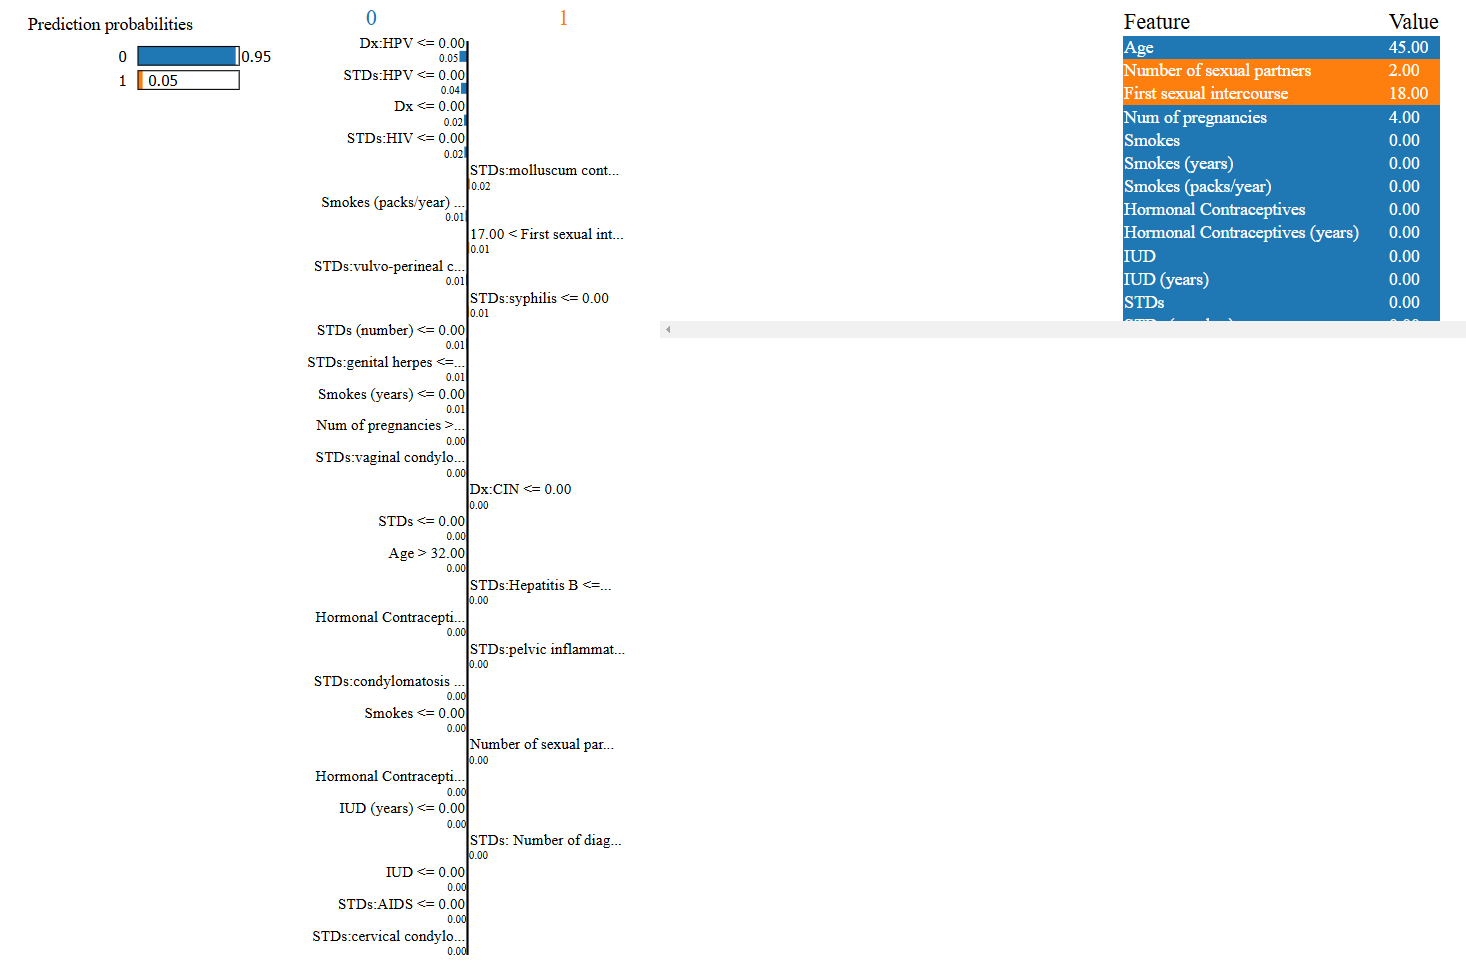
\includegraphics[width=1\textwidth]{images/result1}
	\caption{Based on the H2O AutoML-LIME model prediction probabilities on 29 features for both class ‘0’ and ‘1’ when idx = 120 in the second case, it appears that there is a higher likelihood of belonging to class ‘1’.}
	\label{fig:IDX120}
\end{figure}

\begin{figure}[htbp]
	\centering
	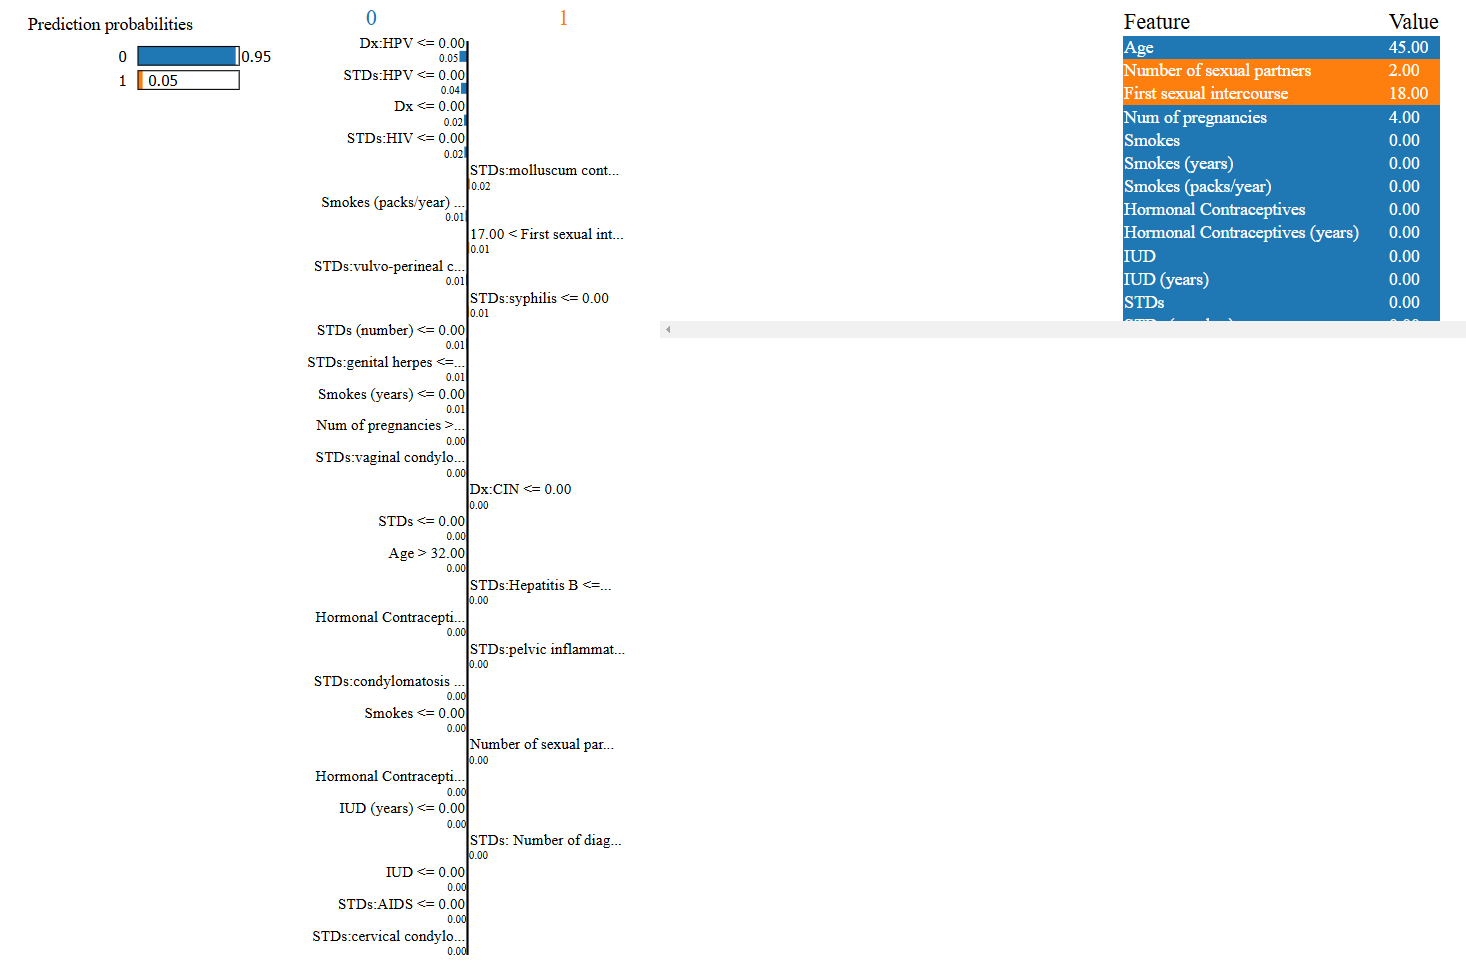
\includegraphics[width=1\textwidth]{images/result1}
	\caption{Based on the H2O AutoML-LIME model prediction probabilities on 29 features for both class ‘0’ and ‘1’ when IDX = 150 in the second case, it appears that there is a higher likelihood of belonging to class ‘1’.}
	\label{fig:IDX150}
\end{figure}

\end{document}
